
\documentclass[letterpaper,12pt]{article} 
\usepackage[utf8]{inputenc}
\usepackage[spanish, activeacute]{babel}
\usepackage{amsmath}
\usepackage{amsfonts}
\usepackage{amssymb} 
\usepackage{algorithm2e}
\usepackage{algorithm}
\usepackage{algorithmic}
\usepackage{graphicx} 			%graficos
\usepackage[colorlinks=true, linkcolor=black, citecolor=black, urlcolor=blue]{hyperref} 	
\usepackage{wrapfig}
\usepackage{enumitem}
\usepackage{fancyhdr}
\usepackage{float}
\usepackage{eurosym}
\usepackage{color}
\usepackage{titling}
\usepackage{lipsum}
\usepackage{tocbibind}
\usepackage{longtable,multirow,booktabs}
\usepackage{multicol}

\usepackage[left=3cm,right=3cm,top=3cm,bottom=4cm]{geometry}		%margenes para documento


\pagestyle{fancy}													% estilo del estlo de pie cabezera


%%% Para las cabeceras
\newcommand{\hsp}{\hspace{20pt}}
\newcommand{\HRule}{\rule{\linewidth}{0.5mm}}
\headheight=50pt


\newcommand{\vacio}{\textcolor{white}{este es un texto que no se vera porque el colorde letra es blanco}} 			%comando para dar un texto 

\definecolor{rojoportada}{rgb}{0.9058 ,0.2980 , 0.23}				%color Rojo para las cabezeras


%====================================Datos del proyecto ======================================

%titulo del proyecto
\title{Aplicacion Multiplataforma de Domotica}				

%%%% AUTORES
\newcommand{\autorUno}{
	Univ. Alexander Mamani Y.\\
	FCyT\\
	Cochabamba\\
	akeymy4@gmail.com.}
\newcommand{\autorDos}{
	Univ. Ismael David.\\
	FCyT\\
	Cochabamba\\
	Isma@gmail.com.}
\newcommand{\autorTres}{
	Univ. Narrieth Felipe P.\\
	FCyT\\
	Cochabamba\\
	narrieth14ajc@gmail.com.}




\begin{document}
	
	
	
	
	
	{%\Large
		
		\newpage
		
		%%%Encabezamiento y pie de página
		%%% También se genera automáticamente
		%%% Mejor no tocarlo mucho.
		\renewcommand{\headrulewidth}{0.5pt}
		\fancyhead[L]{
			\textcolor{rojoportada}{\fontfamily{phv}\fontsize{14}{4}\selectfont{ \textbf{\thetitle}   }}\\
		}
		\fancyhead[R]{
			\textcolor{rojoportada}{\fontfamily{phv}\fontsize{14}{4}\selectfont{ \textbf{SCESI}   }}\\
		}
		
		
		
		
		%=================================pie de pagina==========================
		\renewcommand{\footrulewidth}{0.5pt}
		\fancyfoot[L]{
			\footnotesize SCESI\\
			Sociedad Cientifica de Estudiantes de Sistemas e Informatica\\
			http://www.scesi.org
		}
		\fancyfoot[C]{\vacio}														%hacemos uso del comando que creamo \vacio
		\fancyfoot[R]{\footnotesize Página \thepage}								%numeracion de la pagina					
		\
		\vacio
		\
		
		
		\begin{center}
			\vspace{.5cm}
			{\fontfamily{phv}\fontsize{20}{5}\selectfont{\textsc{\thetitle}}}\\
			[2cm]		
			%importamos una imagen
			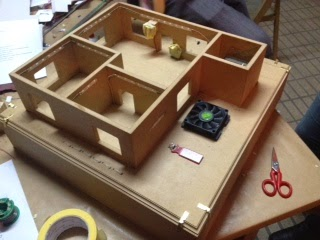
\includegraphics[width=5.5cm]{images/maqueta.jpeg}								
			\\[2cm]
			
			
			%\textcolor{azulportada}	
			
			
			Presentado por :
			\vspace{1.5cm}
			
			\begin{minipage}[b]{5.5cm}
				\begin{center}
					\autorUno
				\end{center}
			\end{minipage} \hfill \begin{minipage}[b]{4cm}
				\begin{center}
					\autorDos
				\end{center}
			\end{minipage} \hfill \begin{minipage}[b]{5cm}
				\begin{center}
					\autorTres
				\end{center}
				
			\end{minipage}\\
			[4cm]
			
			{\fontfamily{phv}\fontsize{12}{3}\selectfont{Cochabamba, 2018}}\\[1cm]
		\end{center}
		
		
		
		\vspace{1cm}
		\ %% Así hago que se abra más espacio entre renglones.
		
		
		
		\tableofcontents
		\newpage
		
		
		
		\section{Introduccion}
		\vspace{1cm}
		
		La Robotica e Informatica en los ultimos años a tenido un gran impacto en los paises en vias de desarrollo gracias a la llegada de tecnologias de fuente Abierta(Open Source), ya sean a nivel de software o hardware  permitiendo que ya no solo las personas  puedan comunicarse entre ellas atravez de la Red(Internet), sino que tambien los dispositivos electronicos.
		
		Del lado de la informatica a lo largo de los ultimos años tambien  empezaron a sugir tecnologias que permiten el desarrolo web de forma mas eficiente, eficaz y sencilla. Permitiendo tanto a desarrolladores como clientes tener acceso  a la Red(internet).
		
		%Tambien si hablamos de Domotica, no podemos dejar a un lado a las IA's( Inteligencia Artifical ), que el los ultimos años se a puesto de moda, debido que permite la solucion de varios problemas cotidianos.
		
		La union de estas tecnologias mensionadas dan origen a lo que conocemos como "Domotica". Que es nada menos que la automatizacion inteligente de un vivienda, que permite una gestión eficiente del uso de la energía, seguridad y confort, además de comunicación entre el usuario y un sistema. 
		
		Este proyecto pretende dar a conocer el desarrollo, implementacion  y despliegue de una Aplicacion Movil multiplataforma de Domotica, usando las tecnologias ya mensionadas.
		
		
		\section{Planteamiento del problema}
		\subsection{Antecedentes}
		
		Uno de los más importantes entornos de una persona es su hogar, es donde  descansamos,  pensamos, crecemos, aprendemos,  envejecemos, disfrutamos y convivimos  junto con nuestra familia y seres queridos, es en donde queremos  vivir con seguridad y privacidad, ir  a dormir  con la tranquilidad de que algo o alguien permanezca siempre alerta a nuestro servicio o que al  salir de vacaciones no tengamos la preocupación que sucederá en nuestra ausencia.  Que al llegar a casa  nunca la encontremos en penumbras , que  encontremos un ambiente agradable de acuerdo a nuestras preferencias,  con más confort,    no solo controlar desde la palma de la mano la TV o reproductores de video  sino también  la iluminación, persianas, liberándonos de tareas repetitivas ( encender las luces cuando anochece,  encender el  purificador de aire , el sistema de riego del jardín, etc.) .
		
		Tambien se hace claro que dentro de este grupo de la población es frecuente encontrarse con personas que presentan  dificultades de interacción con los objetos del hogar, como consecuencia directa o indirecta de la condición particular del individuo. Es así, que para las personas afectadas por discapacidades transitorias  o  con alguna discapacidad motora, el accionar cotidiano de la vivienda puede tornarse en una labor complicada. Labores sencillas, como presionar el interruptor de una luz, abrir una puerta o ventana, utilizar una toma de corriente o alcanzar un control remoto, pueden transformarse en tareas complicadas 
		
		
		
		
		\subsection{Justificacion}
		
		\subsubsection{Situacion sin Proyecto}
		
		Sin la realización de este proyecto, es probable que los sistemas de domótica  en paises en vias de desarrollo tarden en madurar, lo suficiente como para presentarse como una alternativa de ayuda real para las personas discapacitadas, haciendo que los problemas cotidianos que éstas presentan, al interactuar en el ambiente de su casa, queden sin resolver, como tambien la falta de seguridad y confort en las viviendas de paises en vias de desarrollo.
		
		Con la inseguridad que existe en las calles, es dificil poder tener una completa seguridad de la vivienda.
		Tener vigilada la vivienda es algo muy importante en estos tiempos debido a la violencia que existen en algunos hogares.
		
		\subsubsection{Situacion con Proyecto}
		El beneficio de este sistema es que permitirá a la persona discapacitada, aumentar su grado de autonomía y reducir la necesidad de supervisión constante, mejorando de esta forma su calidad de vida.  Además, el sistema será de relativamente bajo costo, permitirá la utilización, dentro de lo posible, de los dispositivos que ya se encuentran en el hogar, lo cual reducirá los requerimientos de nueva infraestructura y se plantea como un sistema de “Arquitectura Abierta”, lo que permitirá su duplicación y  utilización parcial o total por cualquier persona que lo necesite. 
		
		Ayudar con la vigilancia de la vivienda, monitorizar el movimiento existente dentro de ella.
		
		
		\section{Objetivos}
		
		
		
		
		\subsection{Objetivo General}
		
		Diseñar un Aplicacion Movil Multiplataforma de Domotica que permita el control de  iluminacion y accionamiento de puertas de los distintos dormitorios.
		Asi tambien manejar la ventilacion mediante lecturas de humedad y temperatura del ambiente. Tambien contara con un sencillo control de alarma para la detección de intrusos, con video vigilancia(Streaming)  y detection de CO2( Gas )\\\\
		Para todos estos aspectos se pretende crear una aplicacion movil multiplataforma, amigable que permita el control y monitoreo de varias viviendas.
		
		
		\subsection{Objetivos Especificos}
		
		\subsubsection{Electronica del proyecto}
		
		\begin{itemize}
			
			\item Diseñar circuito de conexion y alimentacion de sensores y servomotores para una placa de circuitos impreso (PCB) utilizando el programa de software libre Kicad.
			
			\item Quemar diseño del circuito de conexion y alimentacion de sensores y servomotores en una placa de circuito  impreso (PCB).
			
			\item Soldar componentes electronicos en la placa de circuito impreso (PCB) realizada.
			
			\item Armar y añadir al circuito impreso los sensores y servomotores 
			
			\item Instalacion de la pi camera en la Raspberry
			
		\end{itemize}
		
		
		\subsubsection{Informatica del proyecto}
		
		\begin{itemize}
			\item Programacion del firmware del control principal del la casa(Raspberry)
			\begin{list}{}{}
				\item Programacion del modulo de control de servomotores(\textbf{Puertas}).
				\item Programacion del modulo del sensor de temperatura y humedad.
				\item Programacion del modulo del sensor de presencia (PIR) para la deteccion de presencia.
				\item Programacion del modulo receptor de comandos  Seriales \textbf{Arduino-Raspberry}.
				\item Programacion del modulo para eventos listener \textbf{Raspberry-Firebase}.
				\item Programacion del modulo para la pi camera(Streaming) en la \textbf{Raspberry}.
			\end{list}
			
			\item Programacion de una app movil que permita controlar y monitorear varias viviendas al mismo momento. 
			
			\item Interfaces tanto para usuarios y administradores(con los permisos correspondientes).
			
			\item Implementacion de tecnologias como \textbf{firebase} para la interaccion de datos en tiempo real.
			
			\item Implementacion de tecnologias como React Native  para obtener una aplicacion movil multiplataforma para dispositivos moviles, IOs, Android y Windows phone.
			%\item Uso del microfono del celular para el facil uso de la aplicacion
			
			%%\item Entrenamiento de una IA(Inteligencia Artificial) que permitira el reconocimiento de ciertos comandos de voz en dispositivos moviles
			
			\item Configuracion de la app para la visualizacion de Streaming 
			
		\end{itemize}
		
		
		
		
		\section{Hipotesis}
		
		Presentar las oportunidades que podemos aprovechar automatizando los servicios de viviendas, además de la viabilidad de la implementación de dichos sistemas y por consecuente las ventajas que obtenemos al emplearlos.
		
		Liberar el proyecto bajo una licencia de open source Hardware y Software libre que impulsara el desarrollo tecnologico en la materia de Domotica en Bolivia y paises en vias de desarrollo.
		
		Se logrará reducir el consumo energético, integrando los sistemas inteligentes en los servicios tanto de las viviendas, así como de los edificios.
		
		Podremos lograr mayor confort para el usuario, además de proporcionarle mayor seguridad tanto a él como a la vivienda, edificio.
		
		Presentaremos las oportunidades que podemos aprovechar automatizando los servicios de las viviendas, además de la viabilidad de la implementación de dichos sistemas y por consecuente las ventajas que obtenemos al emplearlos.
		
		\section{Novedad y aporte cientifico}
		
		El aporte cientifico del proyecto consiste en la liberacion del codigo fuente de la aplicacion movil multiplataforma , que permite la administracion y control de usuario y viviendas,  el firmware del microcontrolador  arduino y Raspberry, los esquematicos, diseños del circuito realizado y configuracion basica de una vivienda.\\
		
		La novedad por la parte electronica radica en la elaboracion de un circuto para el control de una vivienda usando herramientas de software libre y open source como: Kicad, Arduino IDE, Raspian, Raspberry, y python.\\
		
		La novedad por la parte informatica radica en la elaboracio de una aplicacion movil multiplataforma usando tecnologias como React Native y Django para el Backend. Tambien cabe resaltar el uso  Firebase con su base de datos en tiempo real. Uso de los recursos del dispositivo movil como el microfono para una mayor facilidad de uso.\\
		
		
		%%El uso de una IA(Inteligencia Artificial) para el reconocimiento de un comando de voz.
		
		
		\section{Desarrolo del proyecto}
		El metodo de desarrollo comprende de 2 areas especificas de trabajo que daran como resaltado la interaccion entre la informatica y electronica la vivienda.
		
		
		\subsection{App Movil}
		
		Consiste en un aplicacion movil multiplataforma desarrollada con las siguientes tecnlogias Django, React Native, Firebase y SQLite3.
		Se restringira el uso de la app con diferentes permisos, tanto para usuarios como para administradores.
		
		En el lado del Backend tenemos a Django un framework que maneja la administracion de usuarios, datos de los mismos, autentificacion, manejos de las urls para las transmisiones de Streaming, manejo de contenido multimedia, y seguridad atravez de sus middlewares.
		
		Para el lado del frontend se uso React Native debido a su portabilidad en dispositivos Android, IOs y Windows phone.
		
		La aplicacion movil multiplataforma es capaz de modificar la estructura de estados de una vivenda(Luces, Puertas, Sensores, ..etc), la cual esta una base de datos en tiempo real  en Firebase.
		
		Este modelo de comunicion permite administrar varios servers (Raspberrys) en tiempo real,  separamos la funcionalidad de la aplicacion con el Firmware de cada server (Raspberry).
		
		La forma de interaccion  entre la aplicacion movil  multiplataforma y un usuario consiste en el modelo  cliente-servidor. donde el cliente  envia peticiones http al servidor de firebase, el cual tiene almacenado estados de su vivenda. Una vez el servidor de firebase datecta un cambio en la estructura de esa vivienda  este informa a su server(Raspberry) y este modifica uno o varios estados(Enciender Luces, Activa Alarma, Abrir Garaje, ..etc).
		
		
		\begin{figure}[h]
			
			\begin{minipage}[t]{17cm}
				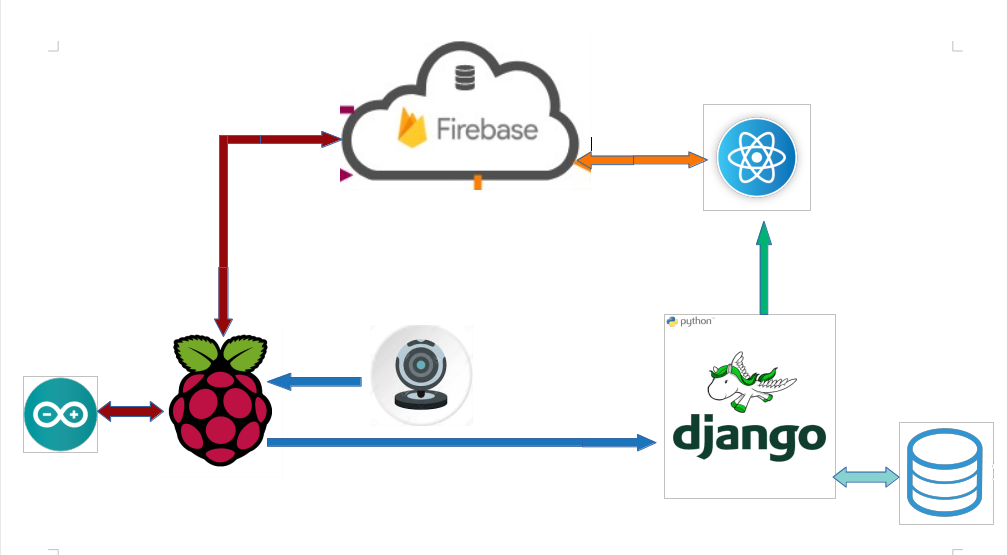
\includegraphics[width=15cm]{images/esquema1.png}	 %importamos una imagen
				\caption{ Esquema de proyecto }
			\end{minipage}
			
		\end{figure}
		
		
		\subsection{Firmware}
		
		Consiste en la parte del software que controla servomotores y sensores de una vivienda. Esto es controlado atravez del SDK de firebase,  el cual permite al server informarse si hubo un cambio en su base de datos o modifcar la misma. 
		
		El mismo se encuentra con Raspian como S.O.  en la Raspberry  y Arduino en el microcontrolador .\\
		
		Debido a que los GPIOS de una Raspberry no tienen entradas analogicas se opto por usar Arduino para las lecturas de los siguente sensores: LDR( Fotoresistor ) y MQ135(sensor  de calidad de aire), este firmware  cuenta con las siguientes funcionalidades:
		
		\begin{itemize}
			\item Comunicaion
			\begin{itemize}
				\item escucha cambios de estados de firebase
				\item mofifica estados de firebase
			\end{itemize}
			
			\item Servomotores y Actuadores 
			\begin{itemize}
				\item Abrir Puerta
				\item Cerrar Puerta
				\item Enceder Led
				\item Apagar Led
				\item Encender Ventilador
				\item Apagar Ventilador
				\item Encender Alerta
				\item Apagar Alerta
			\end{itemize}
			\item Sensores
			\begin{itemize}
				\item Medir temperatura y humedad
				\item detectar presencia de Gas
				\item detectar presencia de Intrusos
				\item medir el grado de iluminacion de un ambiente
				
			\end{itemize}
			\item Camara	
			\begin{itemize}
				\item transmitir Streaming por un puerto del Server
			\end{itemize}
			
		\end{itemize}
		
		\subsection{Componetes Electronicos}
		Los componentes Electronicos usados para este proyecto fueron:\\\\
		\begin{itemize}
			
			\item \textbf{PCB}
			
			Placa de Circuito Impreso donde  se ubica todos los componestes electronicos que se uso para la realizacion del proyecto
			
			\begin{figure}[h]
				\centering
				\begin{minipage}[t]{5.5cm}
					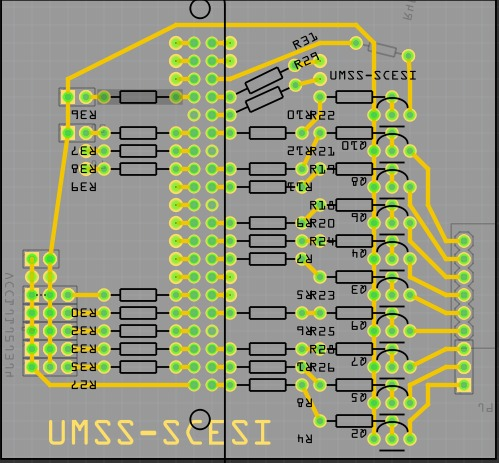
\includegraphics[width=6cm]{images/PCB.jpeg}	 %importamos una imagen
					\caption{ PCB}
				\end{minipage}
				
			\end{figure}
			
			
			\item \textbf{Raspberry Pi}
			
			Mini computador que  posee un System on Chip que contiene un procesador ARM que corre a 700 Mhz, un procesador gráfico VideoCore IV y hasta 512 MG de memoria RAM. Es posible instalar sistema operativos libres a través de una tarjeta SD.
			
			\begin{figure}[h]
				\centering
				\begin{minipage}[t]{5.5cm}
					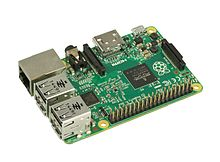
\includegraphics[width=6cm]{images/RaspberryPI.jpg}	 %importamos una imagen
					\caption{ Raspberri Pi}
				\end{minipage}
				
			\end{figure}
			
			
			\item \textbf{Arduino}
			
			Arduino es una plataforma de hardware y software de código abierto, basada en una sencilla placa con entradas y salidas, analógicas y digitales, en un entorno de desarrollo que está basado en el lenguaje de programación Processing. Es decir, una plataforma de código abierto para prototipos electrónicos
			
			\begin{figure}[h]
				\centering
				\begin{minipage}[t]{5cm}
					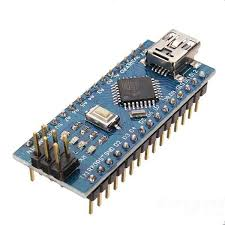
\includegraphics[width=4cm]{images/arduino.jpeg}	 %importamos una imagen
					\caption{ Arduino Nano}
				\end{minipage}
				
			\end{figure}
			
			
			
			
			\item \textbf{Servomotor}
			
			Dispositivos electromecánicos que consisten en un motor eléctrico, un juego de engranes y una tarjeta de control, todo confinado dentro de una carcasa de plástico. sus movimientos son por ancho de pulso y son medidos en grados
			
			\begin{figure}[h]
				\centering
				\begin{minipage}[t]{5cm}
					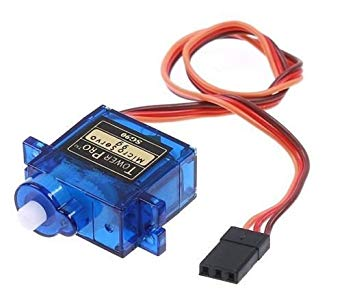
\includegraphics[width=3cm]{images/servo.jpg}	 %importamos una imagen
					\caption{ Servo motor}
				\end{minipage}
				
			\end{figure}
			
			
			\item \textbf{MQ135}
			
			Sensor implementado en la detección de gases peligrosos y en controladores de la calidad del aire. Este sensor es capaz de detectar un amplio rango de gases que incluye: NH3, NOx, alcohol, Benceno, Humo y CO2.
			
			\begin{figure}[h]
				\centering
				\begin{minipage}[t]{5cm}
					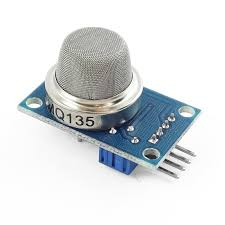
\includegraphics[width=3cm]{images/mq135.jpeg}	 %importamos una imagen
					\caption{Sensor-MQ135 }
				\end{minipage}
				
			\end{figure}
			
			\newpage
			\item \textbf{DTH11}
			
			El DHT11 es un sensor de temperatura y humedad digital de bajo costo. Utiliza un sensor capacitivo de humedad y un termistor para medir el aire circundante, y muestra los datos mediante una señal digital en el pin de datos 
			
			\begin{figure}[h]
				\centering
				\begin{minipage}[t]{5cm}
					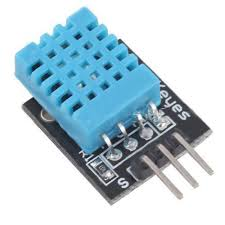
\includegraphics[width=3cm]{images/dht11.jpeg}	 %importamos una imagen
					\caption{Sensor-DHT11 }
				\end{minipage}
				
			\end{figure}
			
			
			\item \textbf{PIR}
			
			Los sensores infrarrojos pasivos (PIR) son dispositivos para la detección de movimiento. Son baratos, pequeños, de baja potencia, y fáciles de usar. Por esta razón son frecuentemente usados en juguetes, aplicaciones domóticas o sistemas de seguridad.
			
			\begin{figure}[h]
				\centering
				\begin{minipage}[t]{3cm}
					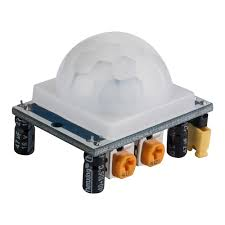
\includegraphics[width=2cm]{images/pir.jpeg}	 %importamos una imagen
					\caption{PIR}
				\end{minipage}
				
			\end{figure}
			
			\newpage
			
			
			\item \textbf{LDR}
			
			Un LDR es un resistor que varía su valor de resistencia eléctrica dependiendo de la cantidad de luz que incide sobre él. Se le llama, también, fotorresistor o fotorresistencia
			
			\begin{figure}[h]
				\centering
				\begin{minipage}[t]{4cm}
					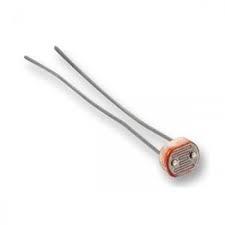
\includegraphics[width=2cm]{images/ldr.jpeg}	 %importamos una imagen
					\caption{Fotoresistor }
				\end{minipage}
				
			\end{figure}
			
			\item \textbf{Pi Camera}
			
			El módulo cámara de 5 megapíxeles esta diseñado específicamente para Raspberry Pi, con un lente de foco fijo. Es capaz de tomar imágenes estáticas de 2592 x 1944, y también es compatible con el formato de video 1080p30, 720p60 y 640x480p60/90.
			
			\begin{figure}[h]
				\centering
				\begin{minipage}[t]{4cm}
					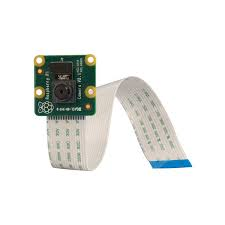
\includegraphics[width=2cm]{images/camerapi.jpeg}	 %importamos una imagen
					\caption{Pi Camera }
				\end{minipage}
				
			\end{figure}
			
			
		\end{itemize}
		
		\section{Metodologias y fuentes}
		
		Para el desarrollo del presente proyecto se uso SCV(Sistemas de control de versiones) como GitHub, el cual permitio el trabajo colaborativo, ya que con el mismo se podia monitorear el avanze del proyecto: \\\
		\begin{itemize}
			\item Creacion de un repositorio
			\item add and commit
			\item envio de cambios
			\item branch 
			\item merges
			\item actualizacion y fusion
			
		\end{itemize}
		
		Tambien se uso SCRUM como metodologia de desarrollo Agil: \\\
		\begin{itemize}
			\item Sprint
			
			\item Sprint Planning
			
			\item Daily Scrum
			
			\item Sprint Review
			
			\item Sprint Retrospective
			
		\end{itemize}
		
		
		Para poder discriminar y seleccionar la información, tomamos como fuentes de información primarias a articulos, ensayos y tesis de Sistemas Domoticos realizados.
		
		
		\section{Conclusiones y Recomendaciones}
		A pesar de las tecnologias usadas en el proyecto, aun quedan cabos sueltos que hay que mejorar y resolver,tal es el caso del Streaming, ya que si se logro realizar la transmision, pero es muy lenta y no se logra visualizar con claridad, esto es debido a que usamos el Protocolo Http para la visualizacion y este no fue diseñado para compartir archivos tan pesados como son estos.\\
		
		Se recomienda tambien la implementacion de una IA (Inteligencia Artificial), para el reconocimiento de comando de voz. 
		Que por ahora con la ayuda del React Native hacemos uso del microfono del dispositivo movil
		
		
		%\newpage
		%\section{GLOSARIO DE TÉRMINOS}
		%\subsection{Diccionario}
		%\begin{itemize}
		
		%	\item \textbf{Arduino.- } Arduino es una plataforma de prototipos electrónica de código abierto (open – source) basada en hardware y software flexibles y  fáciles de usar. Está pensado e inspirado en artistas, diseñadores, y estudiantes de computación o robótica
		
		%	\item \textbf{Concurrecia.- } evento cuando  mas de un proceso intentan acceder al mismo recurso 
		
		%	\item \textbf{MVC .- }Arquitectura de software que separa los datos de una aplicación, la interfaz de usuario, y la lógica de control en tres componentes distintos.
		
		%	\item \textbf{Singleton.- } Es un patrón de diseño que permite restringir la creación de objetos pertenecientes a una clase o el valor de un tipo a un único objeto.Su intención consiste en garantizar que una clase solo tenga una instancia y proporcionar un punto de acceso global a ella.
		
		%	\item \textbf{Eficiencia Espacial.- }Cantidad de recursos espaciales ( de  almacén) que un algoritmo consume o necesita para su 	ejecución
		
		%	\item \textbf{SCV.- }  Software que administra el acceso a un conjunto de ficheros, y mantiene un historial de cambios realizados. El control de versiones es útil para guardar cualquier documento que cambie con frecuencia, como código fuente, documentación o ficheros de configuración.
		
		%	\item \textbf{XML.- } XML proviene de eXtensible Markup Language (“Lenguaje de Marcas Extensible”). Se trata de un metalenguaje (un lenguaje que se utiliza para decir algo acerca de otro) extensible de etiquetas que fue desarrollado por el Word Wide Web Consortium (W3C)
		
		%	\item \textbf{Comunicacion Asincrona.- }Es la conexión que se establece entre el cliente y el servidor que permite la transferencia de datos no sincrónica, o sea el cliente puede realizar varias peticiones al servidor sin necesidad de esperar por la respuesta de la primera. 
		
		
		%\end{itemize}
		
		\newpage
		
		
		\section{Bibliografia}
		
		
		
		\begin{thebibliography}{9}
			%\bibitem(Vesperman,2007){Vesperman} J. Vesperman. “Essential CVS”. O’Really Media Inc, 2007.
			\bibitem{React Native}{React Native} https://facebook.github.io/react-native/
			\bibitem{firebase}{Firebase} https://firebase.google.com/docs/
			\bibitem{raspbery}{RaspberryPi} https://www.raspberrypi.org/documentation/
			\bibitem{Arduino}{Arduino} https://www.arduino.cc/en/Tutorial/HomePage
			\bibitem{Django}{Django} https://docs.djangoproject.com/es/2.1/
			\bibitem{Andrade} A. Andrade . "IMPLEMENTACIÓN DEL SISTEMA DE DOMÓTICA EN EL HOGAR". Trabajo de grado presentado como requisito parcial para optar al título: Ingeniero de Sistemas y Telecomunicaciones , Mexico, 2015
			
			\bibitem{Lorente} Santiaglo Lorete . "¿QUÉ ES LA DOMÓTICA?". Ecuador, 2011
			
		\end{thebibliography}
		
		\newpage
		
	\end{document}
	
